<<<<<<< HEAD
\chapter{Testy i ocena wyników}
\label{cha:Testy i ocena wyników}
\section{Test wykrywania koloru znacznika w przestrzeni barw YCbCr} 
\label{sec:Test wykrywania koloru znacznika w przestrzeni barw YCbCr}
W celu zbadania możliwości wykrycia koloru znacznika przygotowano 3~fotografie wykonane kamerą PCAM~5C. Każde ze~zdjęć przedstawia czerwone koło (kształt znacznika był przy tym teście mniej istotny) i~zostało zrobione przy innym oświetleniu.\\
--- Tutaj planuję opis poniższych zdjęć (szczególnie histogramów) wraz z wnioskami, że możliwa jest skuteczna detekcja czerwonego znacznika na podstawie składowej Cr.
\begin{figure}[h]
	\centering
	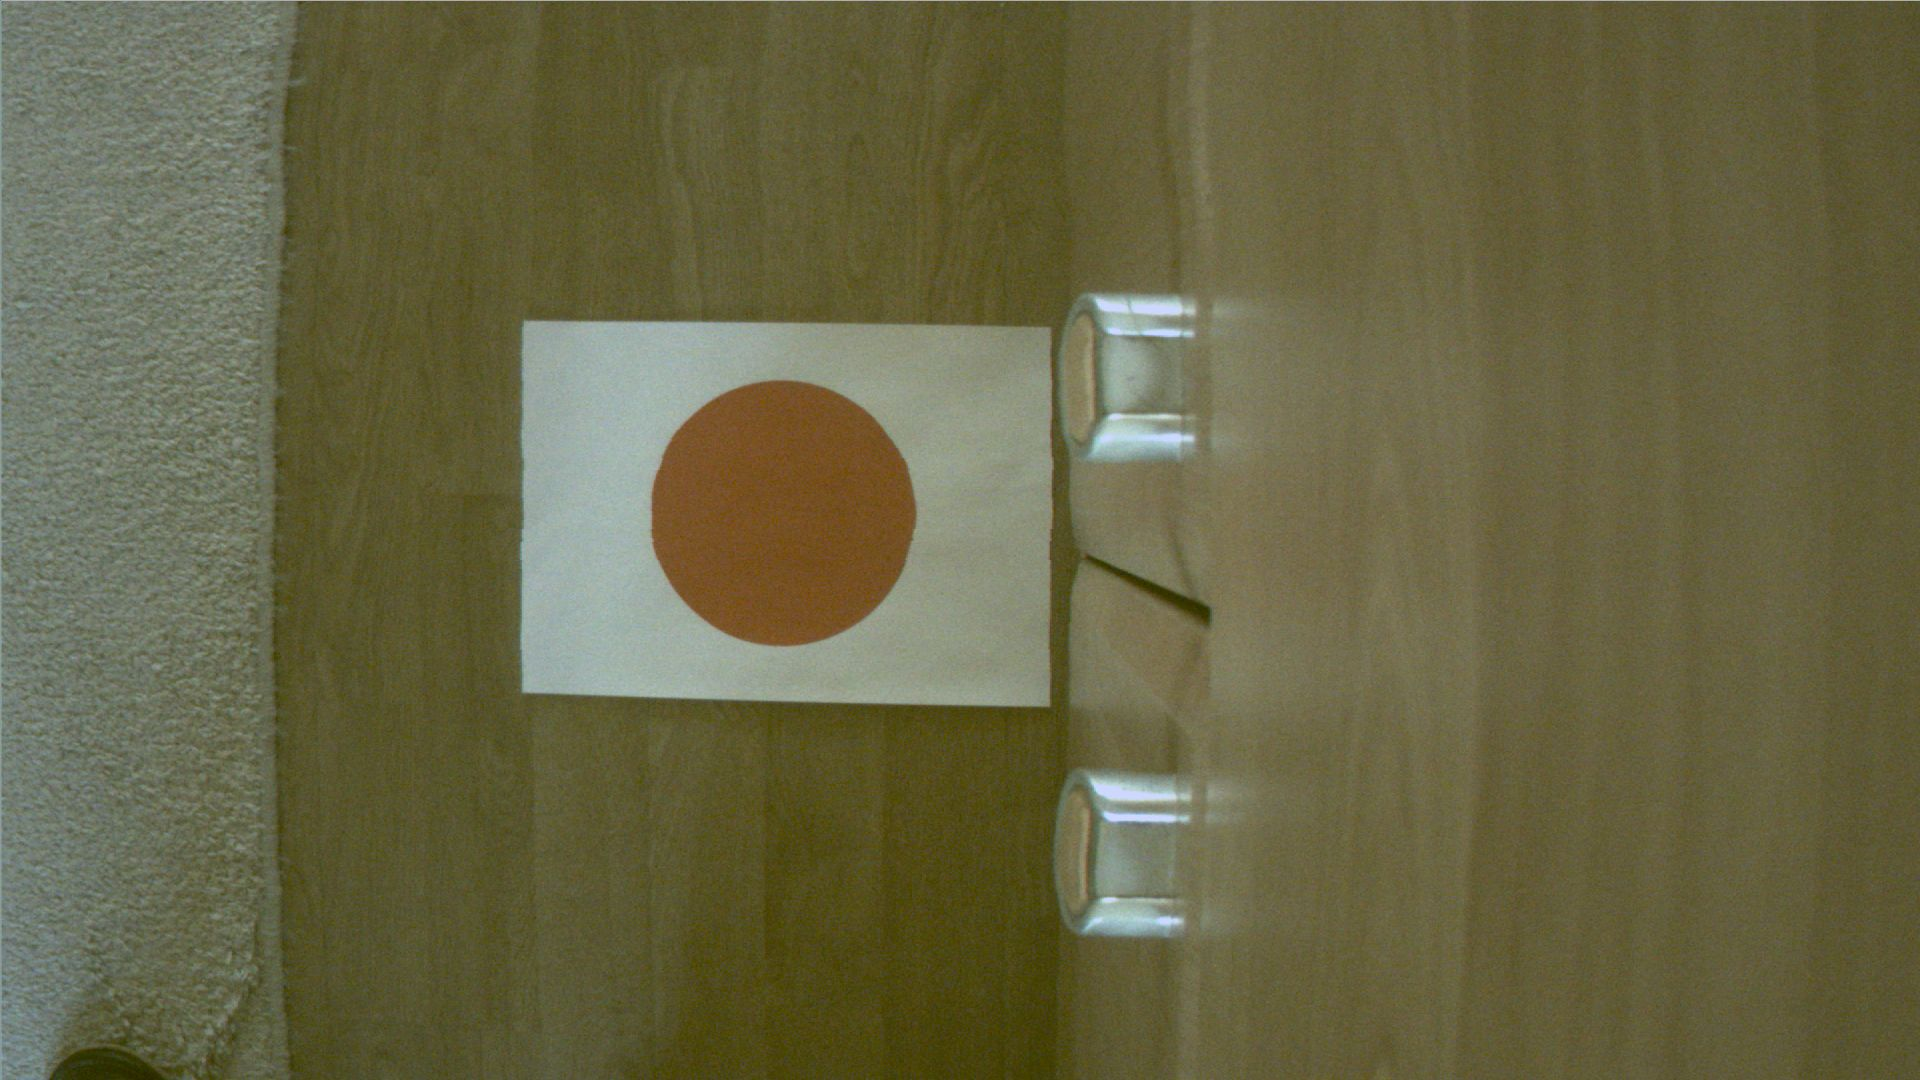
\includegraphics[width=\textwidth]{osw1.jpg}
	\caption{Obraz wykonany przy najmniejszym z badanych oświetleń}
	\label{fig:osw1}
\end{figure}
\begin{figure}[h]
	\centering
	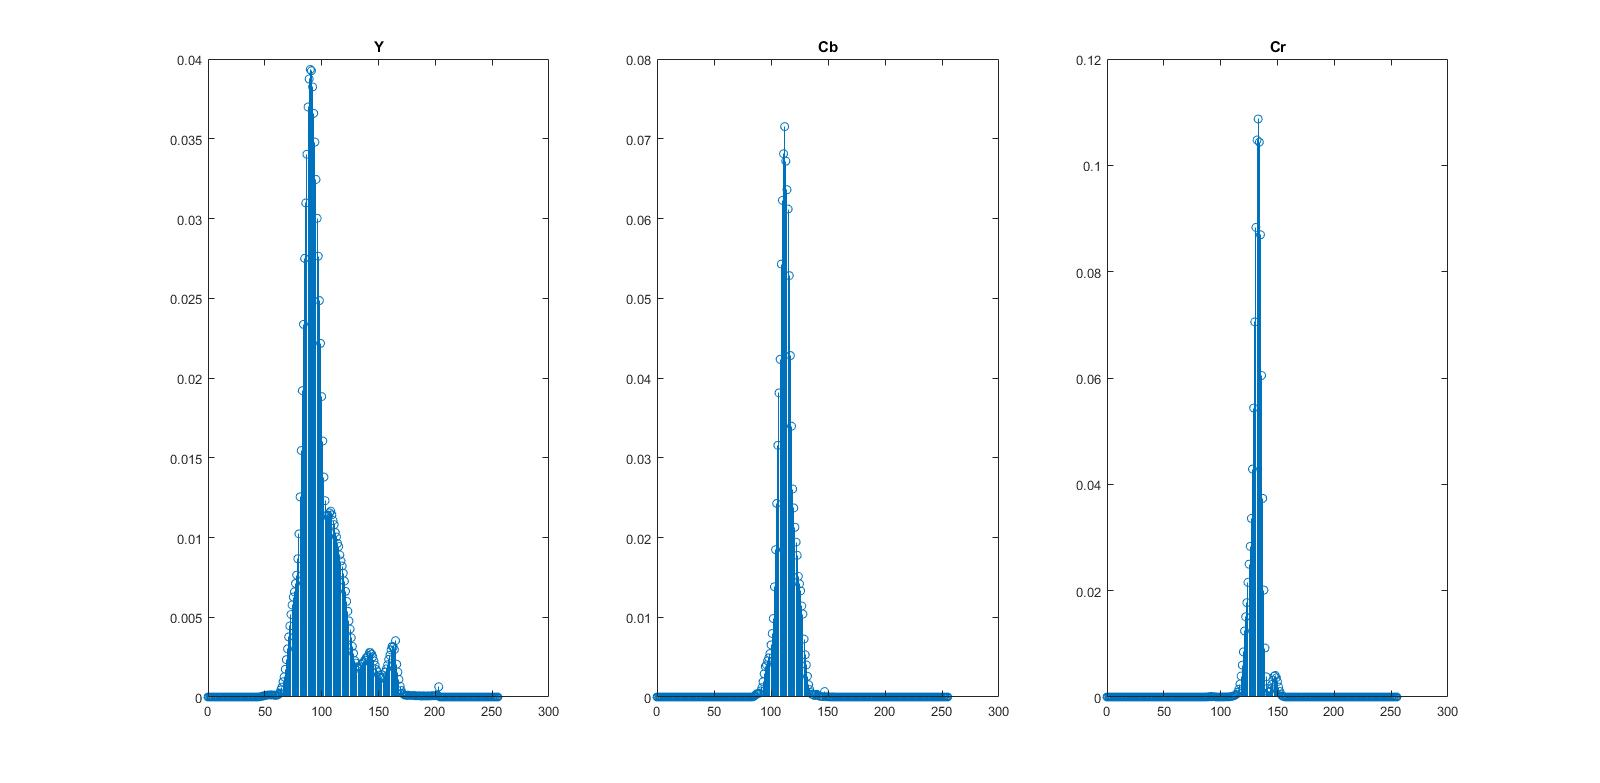
\includegraphics[width=\textwidth]{hist1.jpg}
	\caption{Histogram obrazu wykonanego przy najmniejszym z badanych oświetleń}
	\label{fig:hist1}
\end{figure}
\begin{figure}[h]
	\centering
	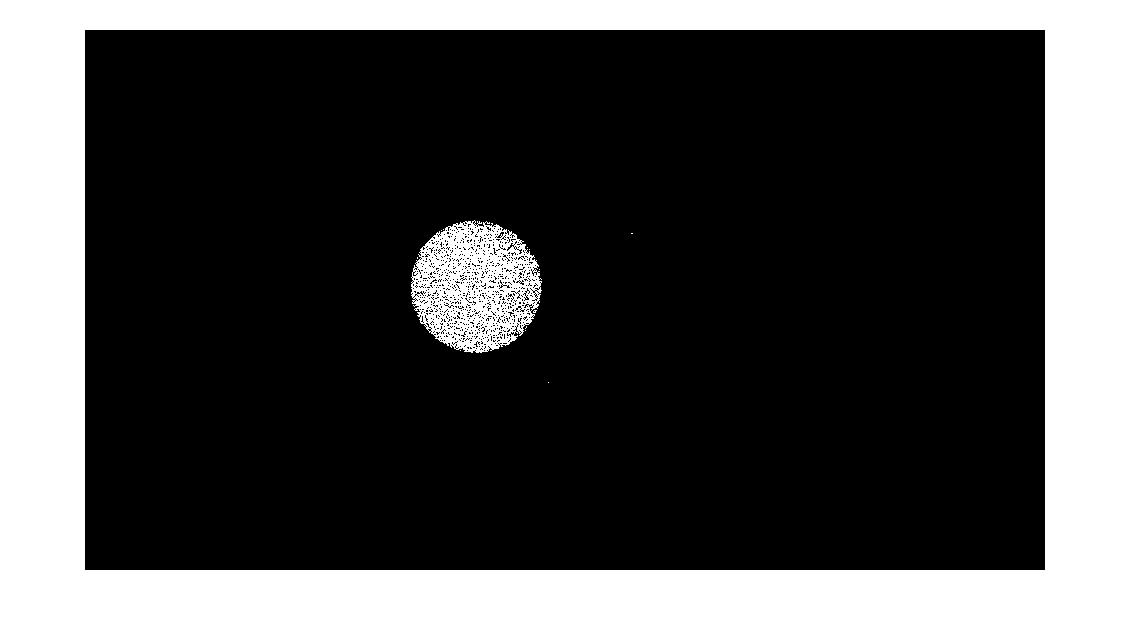
\includegraphics[width=\textwidth]{bin1.jpg}
	\caption{Binaryzacja obrazu wykonanego przy najmniejszym z badanych oświetleń}
	\label{fig:bin1}
\end{figure}
\begin{figure}[h]
	\centering
	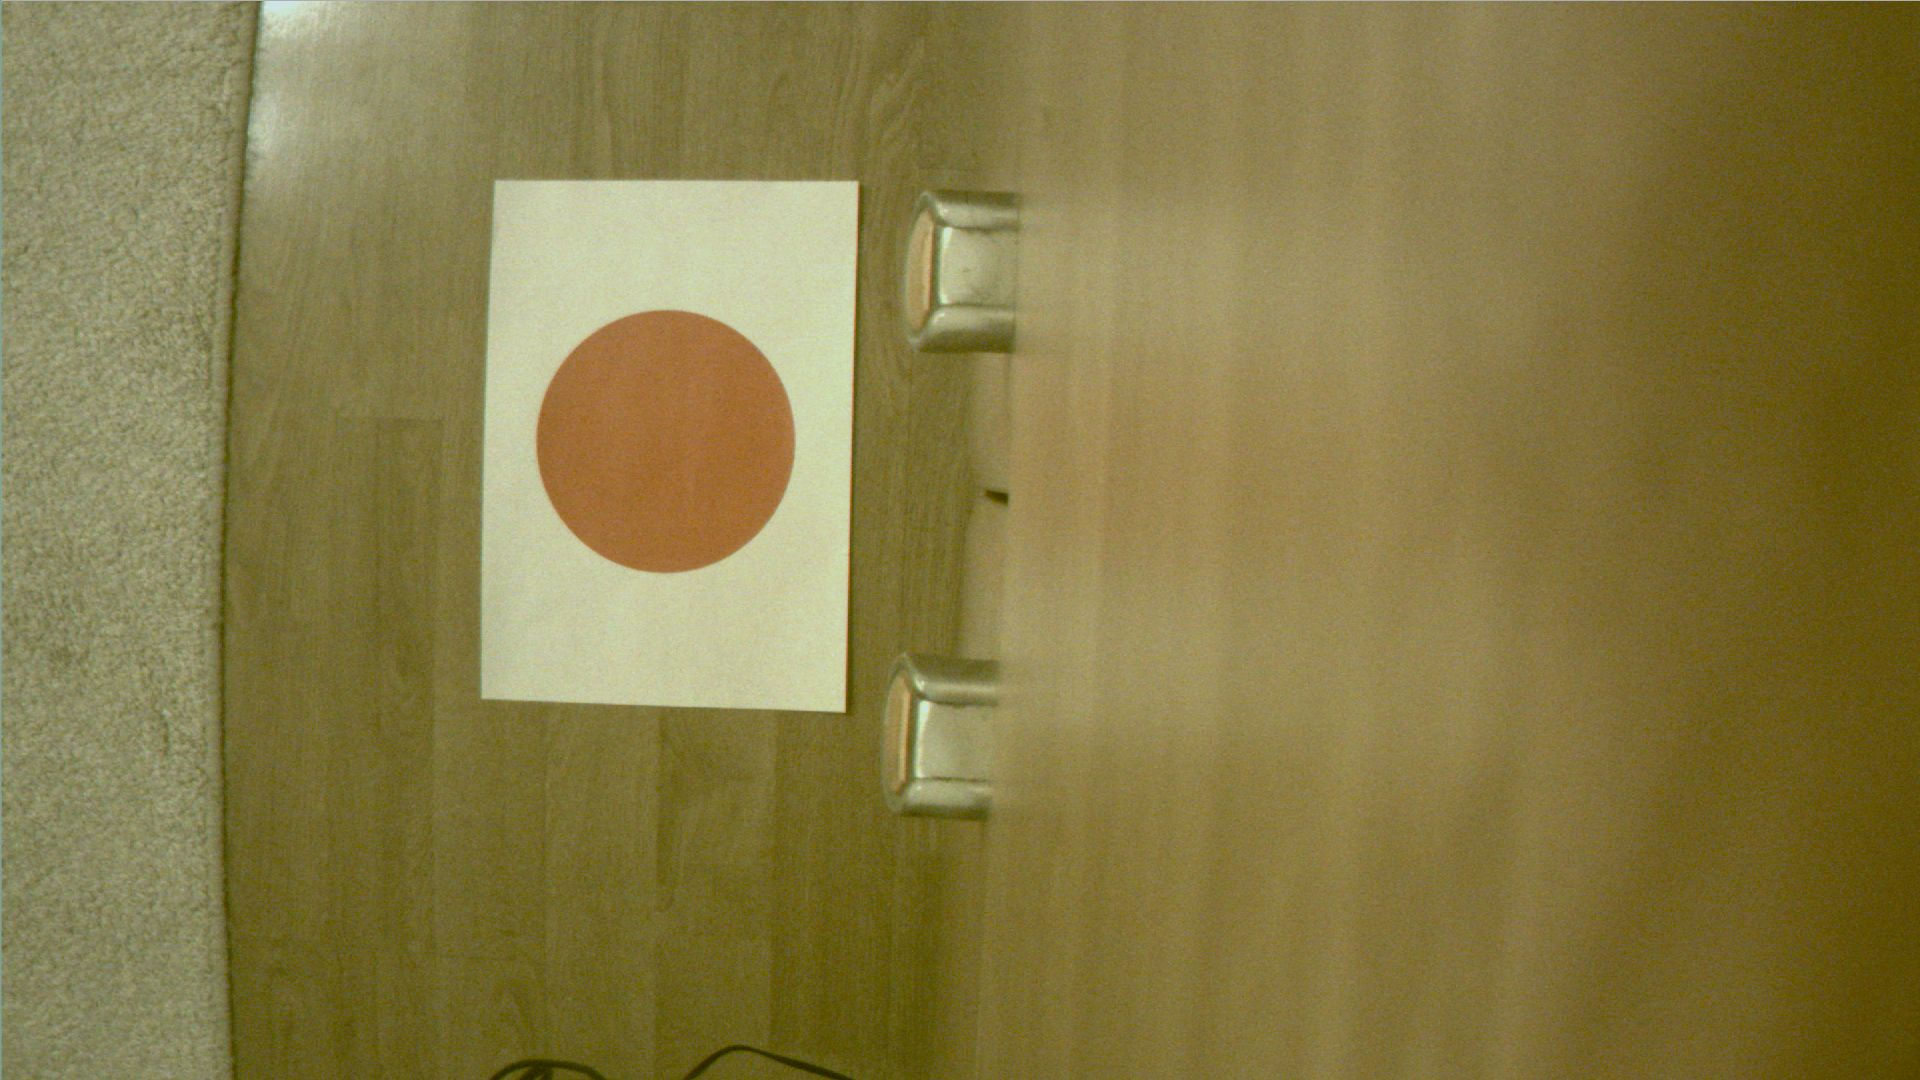
\includegraphics[width=\textwidth]{osw2.jpg}
	\caption{Obraz wykonany przy średnim oświetleniu}
	\label{fig:osw2}
\end{figure}
\begin{figure}[h]
	\centering
	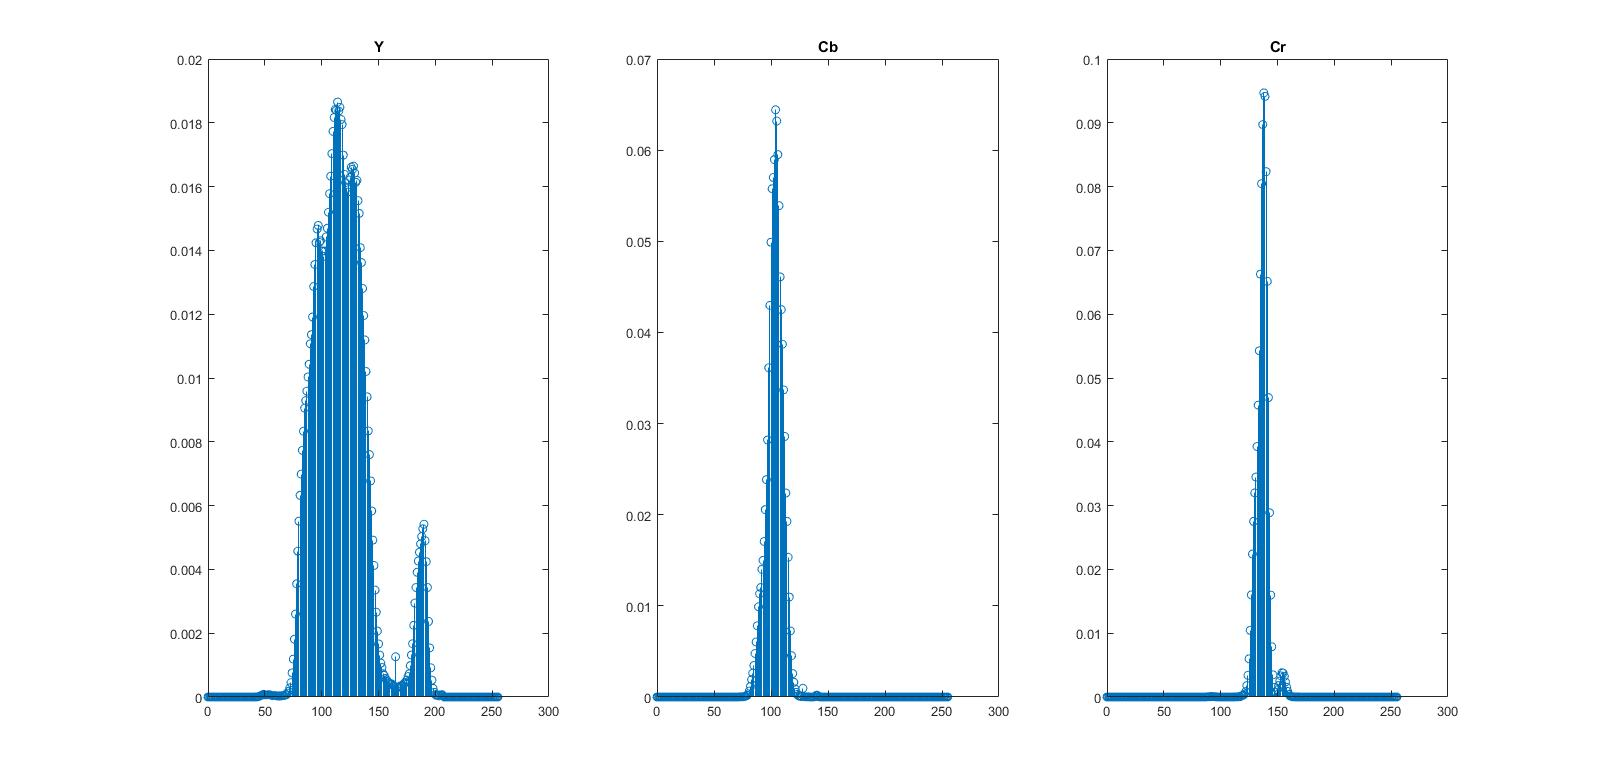
\includegraphics[width=\textwidth]{hist2.jpg}
	\caption{Histogram obrazu wykonanego przy średnim oświetleniu}
	\label{fig:hist2}
\end{figure}
\begin{figure}[h]
	\centering
	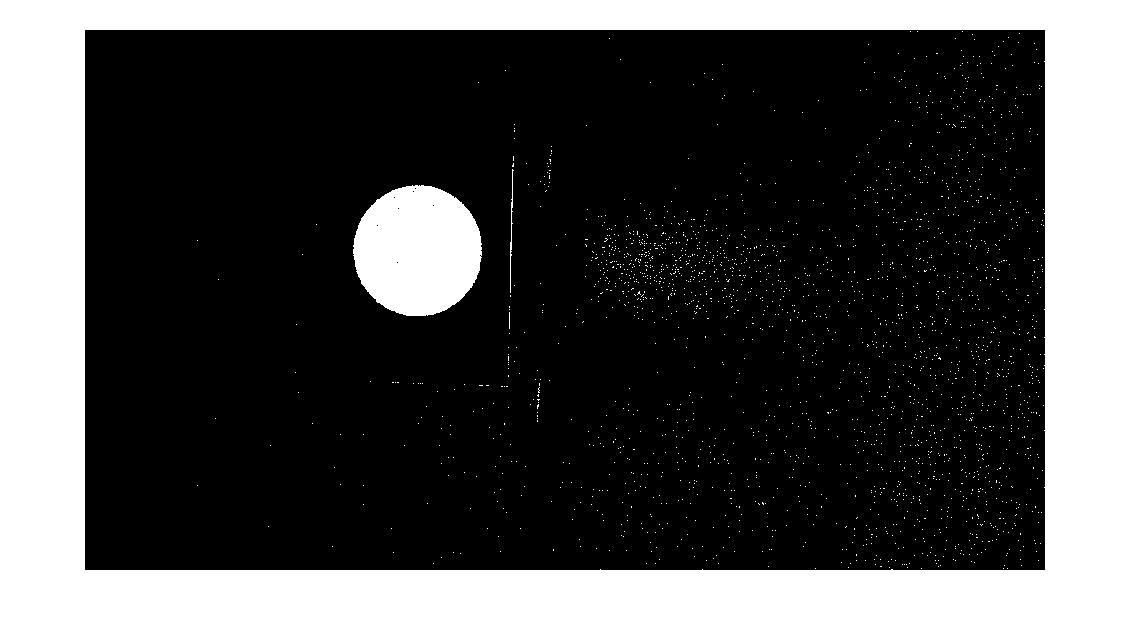
\includegraphics[width=\textwidth]{bin2.jpg}
	\caption{Binaryzacja obrazu wykonanego przy średnim oświetleniu}
	\label{fig:bin2}
\end{figure}
\begin{figure}[h]
	\centering
	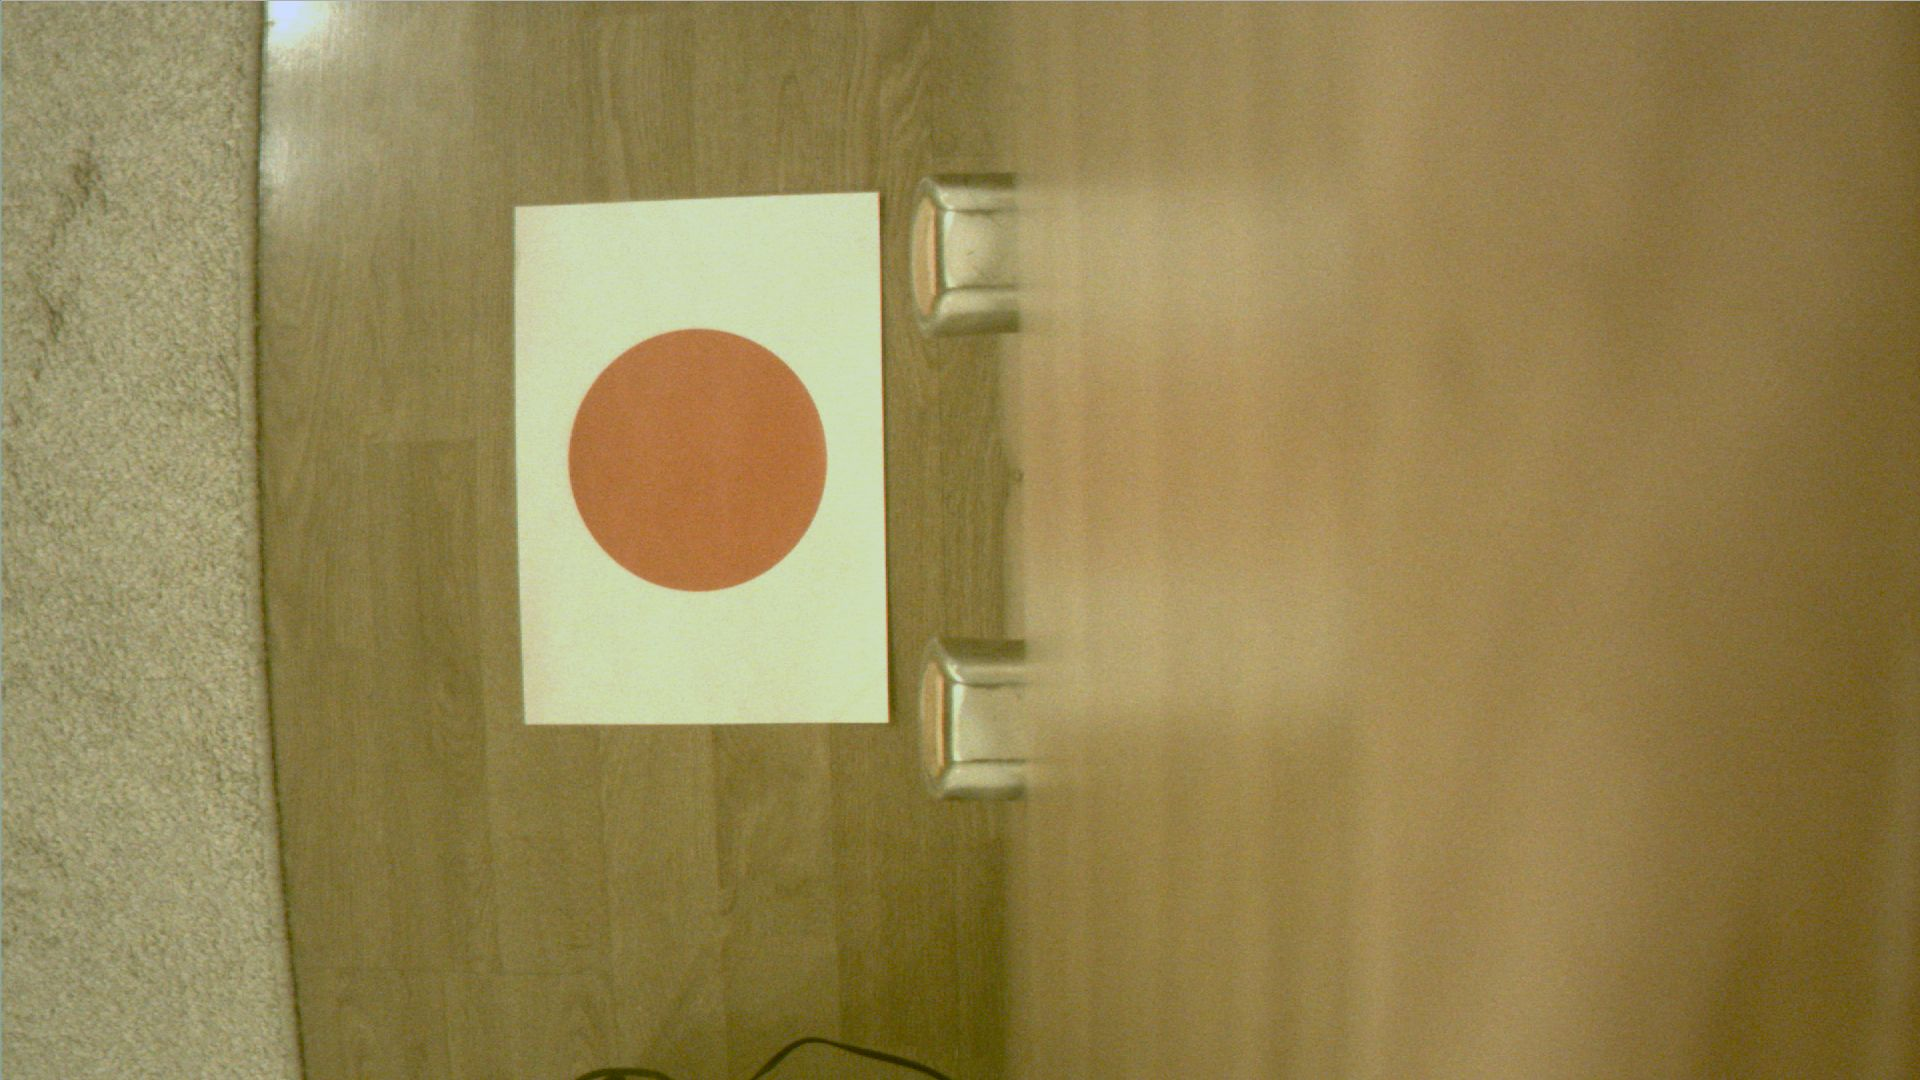
\includegraphics[width=\textwidth]{osw3.jpg}
	\caption{Obraz wykonany przy największym z badanych oświetleń}
	\label{fig:osw3}
\end{figure}
\begin{figure}[h]
	\centering
	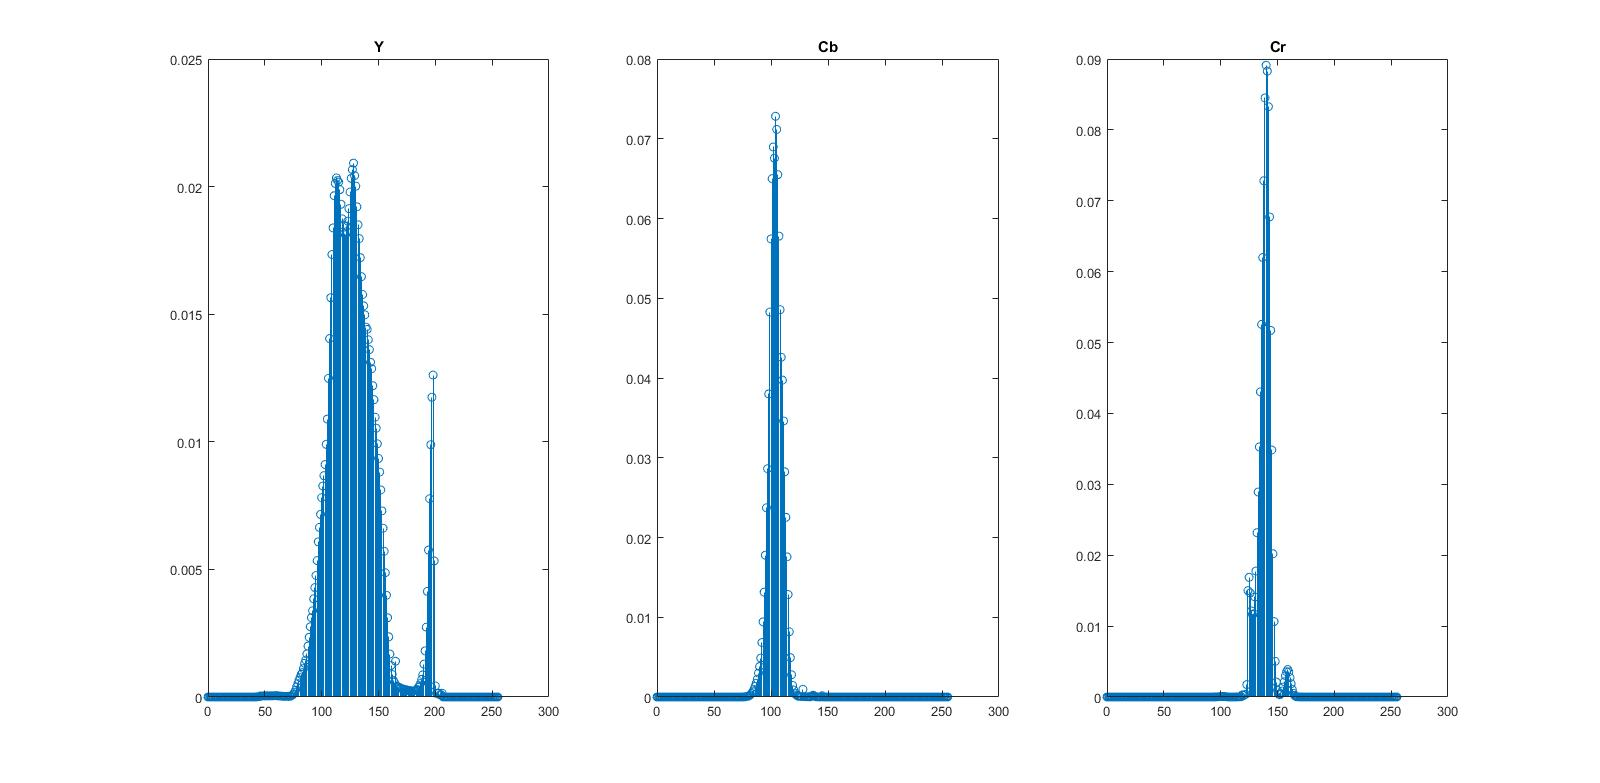
\includegraphics[width=\textwidth]{hist3.jpg}
	\caption{Histogram obrazu wykonanego przy największym z badanych oświetleń}
	\label{fig:hist3}
\end{figure}
\begin{figure}[h]
	\centering
	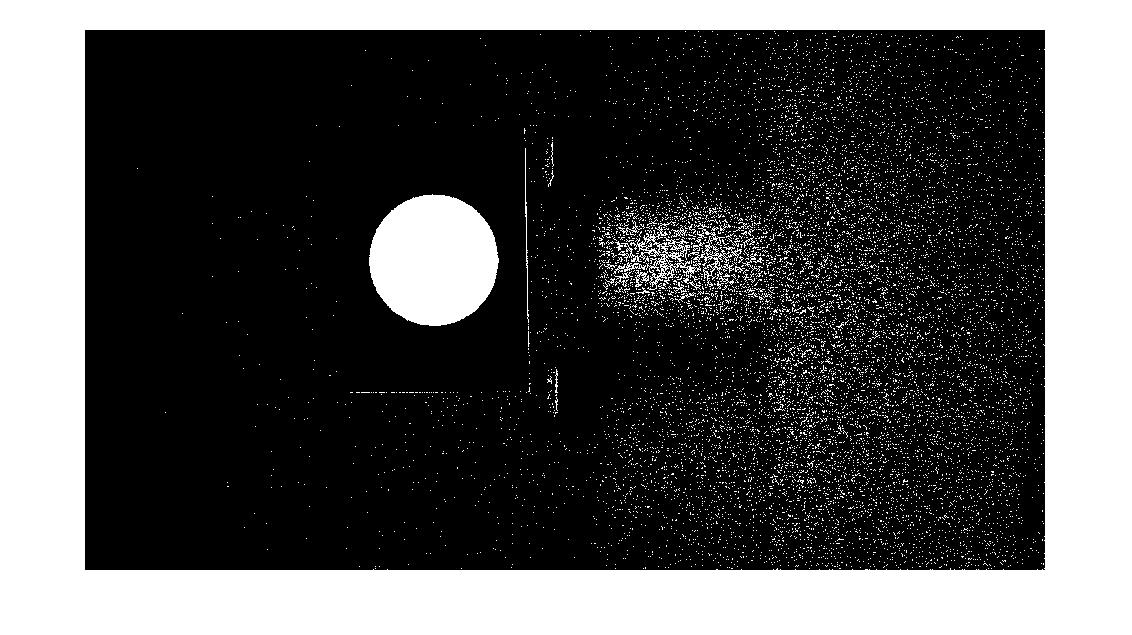
\includegraphics[width=\textwidth]{bin3.jpg}
	\caption{Binaryzacja obrazu wykonanego przy największym z badanych oświetleń}
	\label{fig:bin3}
\end{figure}
\section{Wyznaczenie kąta widzenia kamery przy różnych ustawieniach rozdzielczości}
\label{sec:wyznaczenia_kata_kamery}
Do zbadania kąta widzenia kamery wykorzystano moduł wyznaczający prostopadłe linie przechodzące przez środek obrazu. Następnie umieszczono kamerę na wysokości 49 cm i~skierowano ją w~dół. Odczytanie odległości od~środka obrazu do~jego krawędzi w~poziomie i~pionie pozwoliło na wyznaczenie kątów widzenia kamery. Skorzystano ze wzoru \ref{eq:kat}.
\begin{equation}
\label{eq:kat}
\alpha=\arctan{\frac{l}{h}}
\end{equation}
gdzie:
\begin{eqwhere}[2cm]
	\item[$\alpha$] kąt widzenia kamery,
	\item[$h$] wysokość, na jakiej umieszczona jest kamera,
	\item[$l$] odległość środka obrazu od jego krawędzi.
\end{eqwhere}
Na podstawie obrazu przedstawionego na rysunku \ref{fig:1080p} obliczono kąty widzenia kamery w~pionie i~poziomie dla rozdzielczości 1920 x 1080. Dla rozdzielczości 1280 x 720 skorzystano z~obrazu pokazanego na rysunku \ref{fig:720p}. Korzystając ze wzoru \ref{eq:kat} otrzymano przybliżone wyniki, przedstawione w tabeli \ref{tab:rozdzielczosc}.
\begin{table}[]
	\caption{Wartości kąta widzenia kamery w zależności od rozdzielczości}
	\label{tab:rozdzielczosc}
	\centering
	\begin{tabular}{|c|c|c|}
		\hline
		\begin{tabular}[c]{@{}c@{}}Rozdzielczość\end{tabular} &  Kąt widzenia kamery w pionie w stopniach  &  Kąt widzenia kamery w poziomie w stopniach  \\ \hline
		1920 x 1080                                                                          & 14 & 27 \\ \hline
		1280 x 720                                                                         & 19 & 38 \\ \hline

	\end{tabular}
\end{table}
\begin{figure}[h]
	\centering
	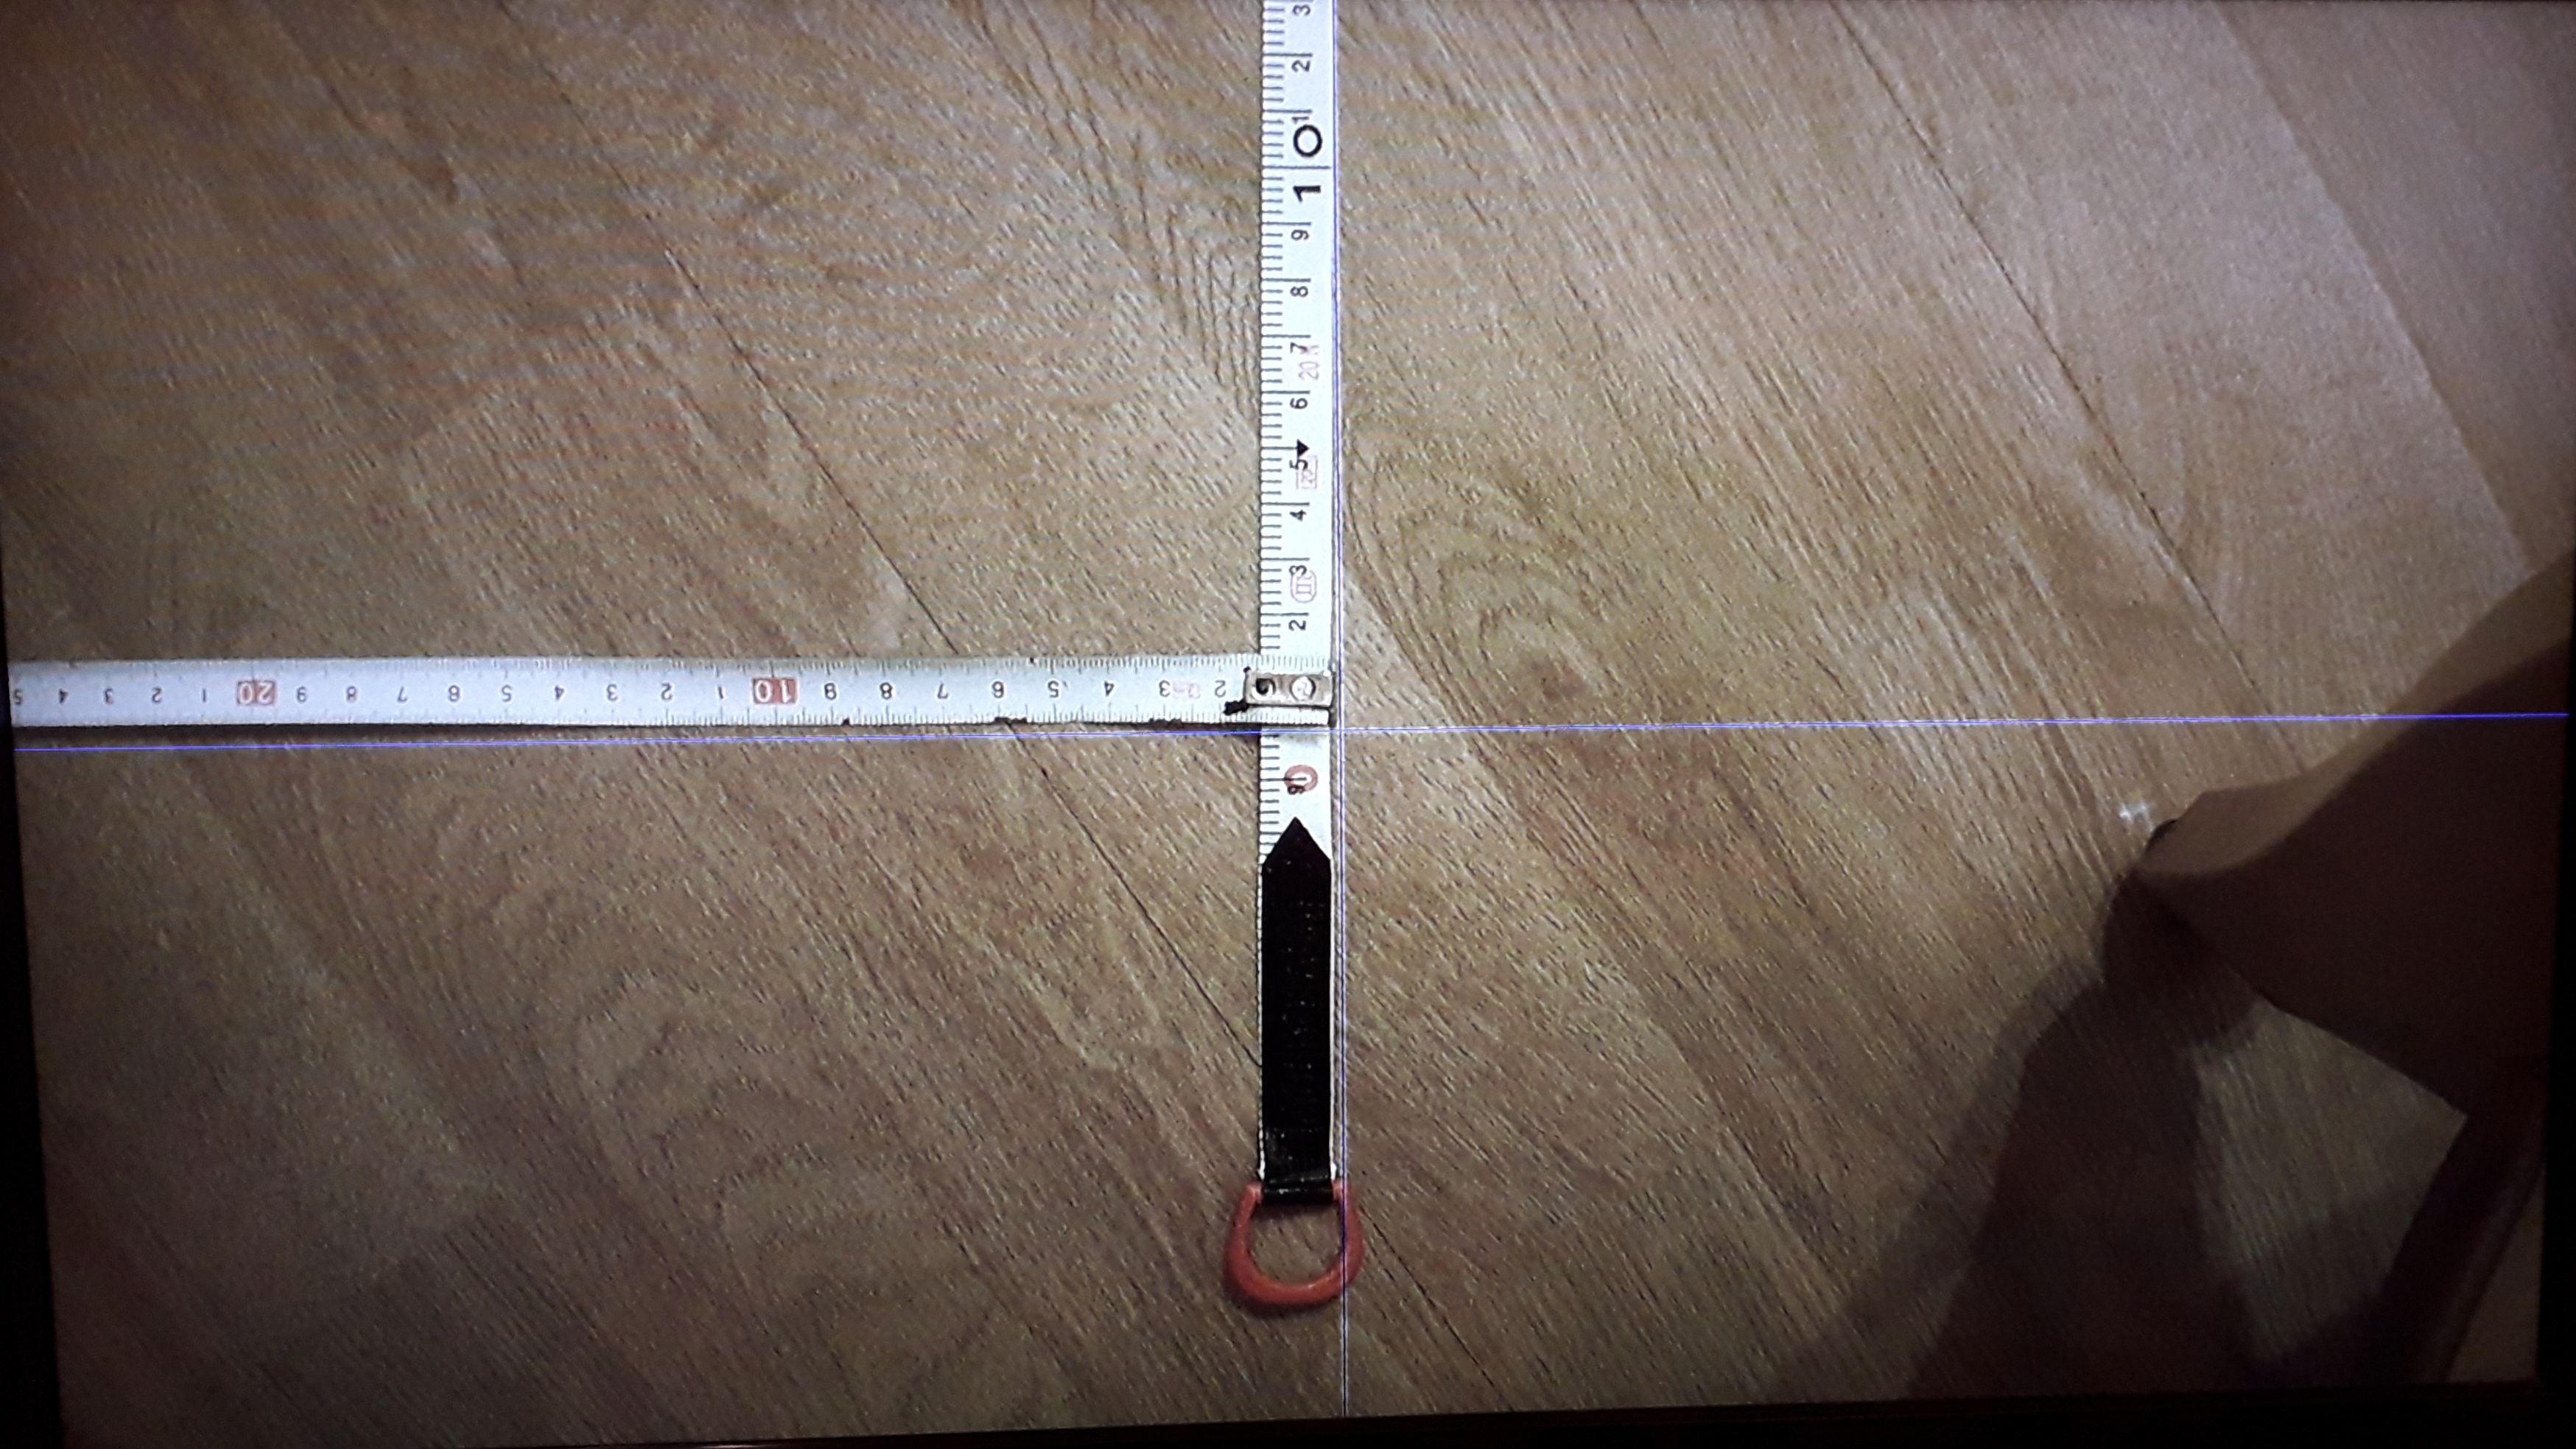
\includegraphics[width=\textwidth]{1080p.jpg}
	\caption{Obraz służący do wyznaczenia kąta widzenia kamery dla rozdzielczości 1920 x 1080.}
	\label{fig:1080p}
\end{figure}
\begin{figure}[h]
	\centering
	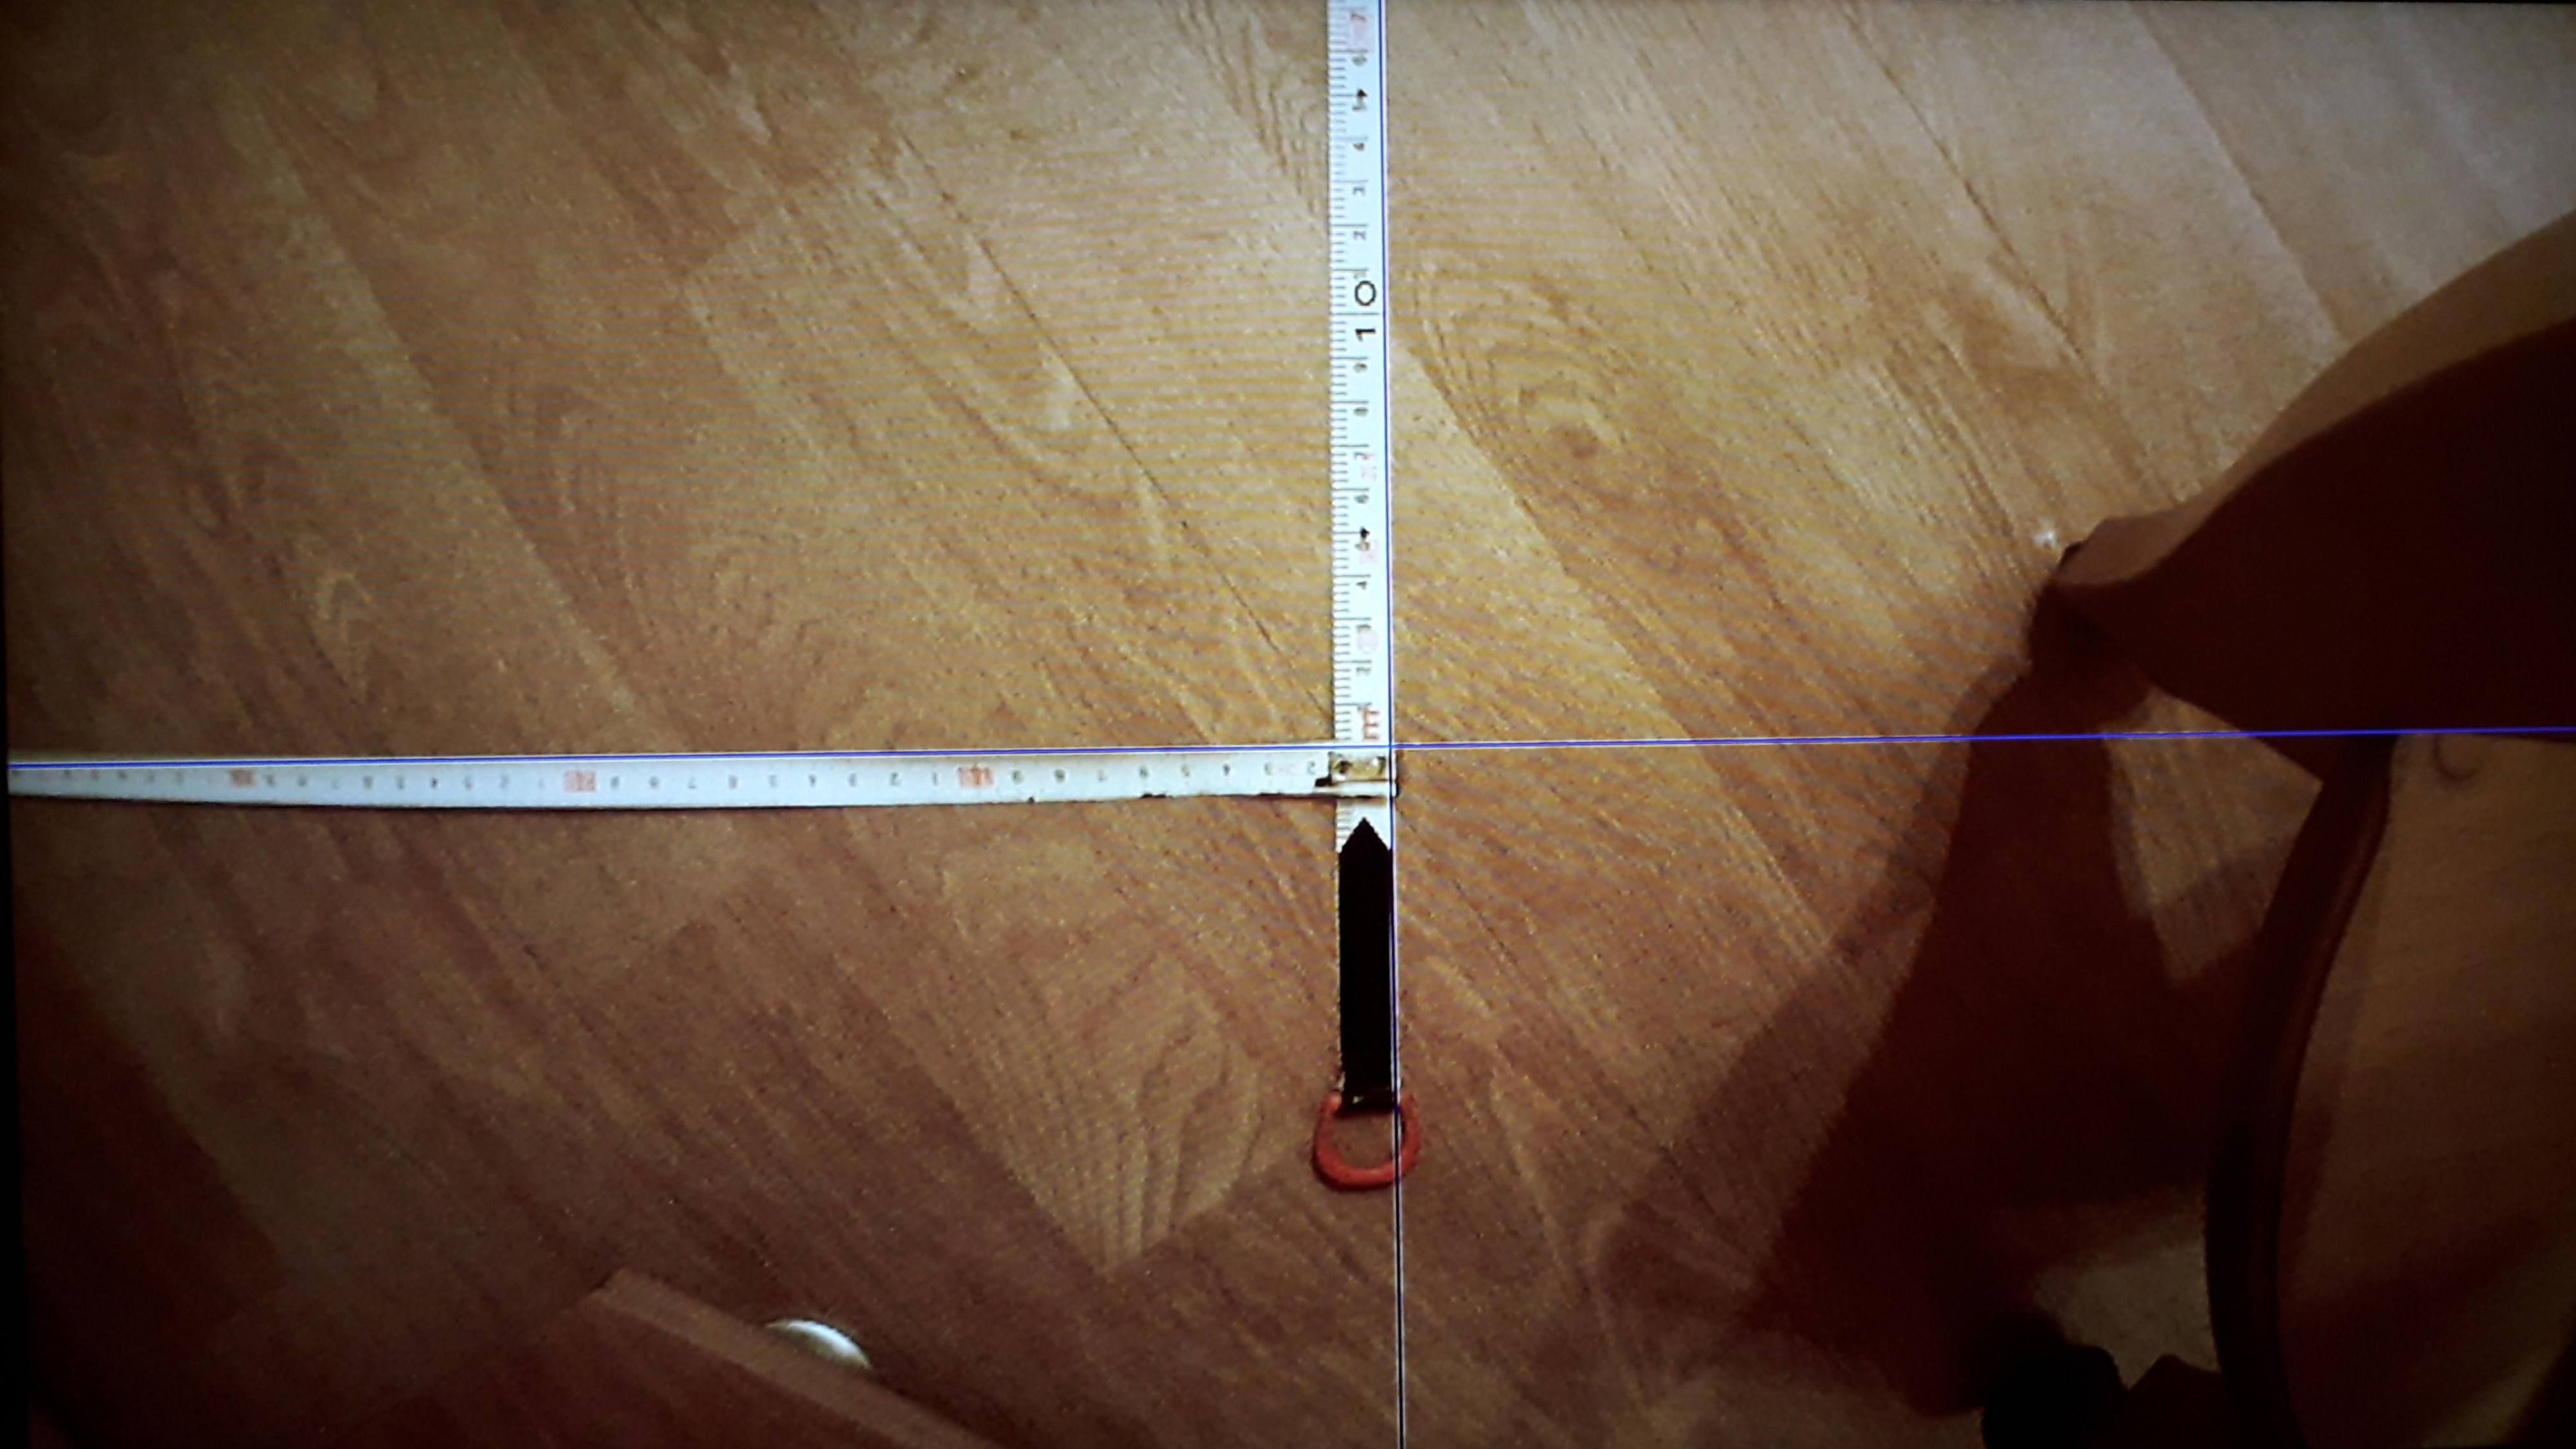
\includegraphics[width=\textwidth]{720p.jpg}
	\caption{Obraz służący do wyznaczenia kąta widzenia kamery dla rozdzielczości 1280 x 720.}
	\label{fig:720p}
\end{figure}

\section{Test detekcji znacznika na obrazie}
\label{sec:Test wydobycia znacznika}
Na rysunku \ref{fig:h} przedstawiono zdjęcie znacznika wykonane z~wysokości jednego metra. Zastosowanie binaryzacji (rysunek \ref{fig:bin}) pozwoliło na oddzielenie znacznika od tła. Na obrazie znajdują się jednak inne niewielkie obszary, które również uzyskały kolor biały. Wykorzystanie mediany spowodowało znaczne zmniejszenie tych obszarów, jednakże na rysunku \ref{fig:median} widoczne są nadal małe grupy białych pikseli nienależących do~markera. Zastosowanie morfologicznego otwarcia, składającego się z~erozji i~dylatacji,  pozwoliło na całkowite wyeliminowanie błędnych białych pikseli. Na~koniec wykorzystano również operację zamknięcia, polegającej na wykonaniu najpierw dylatacji, a potem erozji. Na rysunkach \ref{fig:opened} i \ref{fig:closed}, przedstawiających rezultaty kolejno otwarcia i~zamknięcia, nie widać większych różnic. W~pewnych sytuacjach jednak otwarcie prowadzi do~podziału obiektu na~kilka części. W~takich przypadkach wykonanie zamknięcia może ponownie połączyć obiekty. Może to być istotne w~dalszych pracach nad projektem przy wykorzystaniu indeksacji. 
\begin{figure}[h]
	\centering
	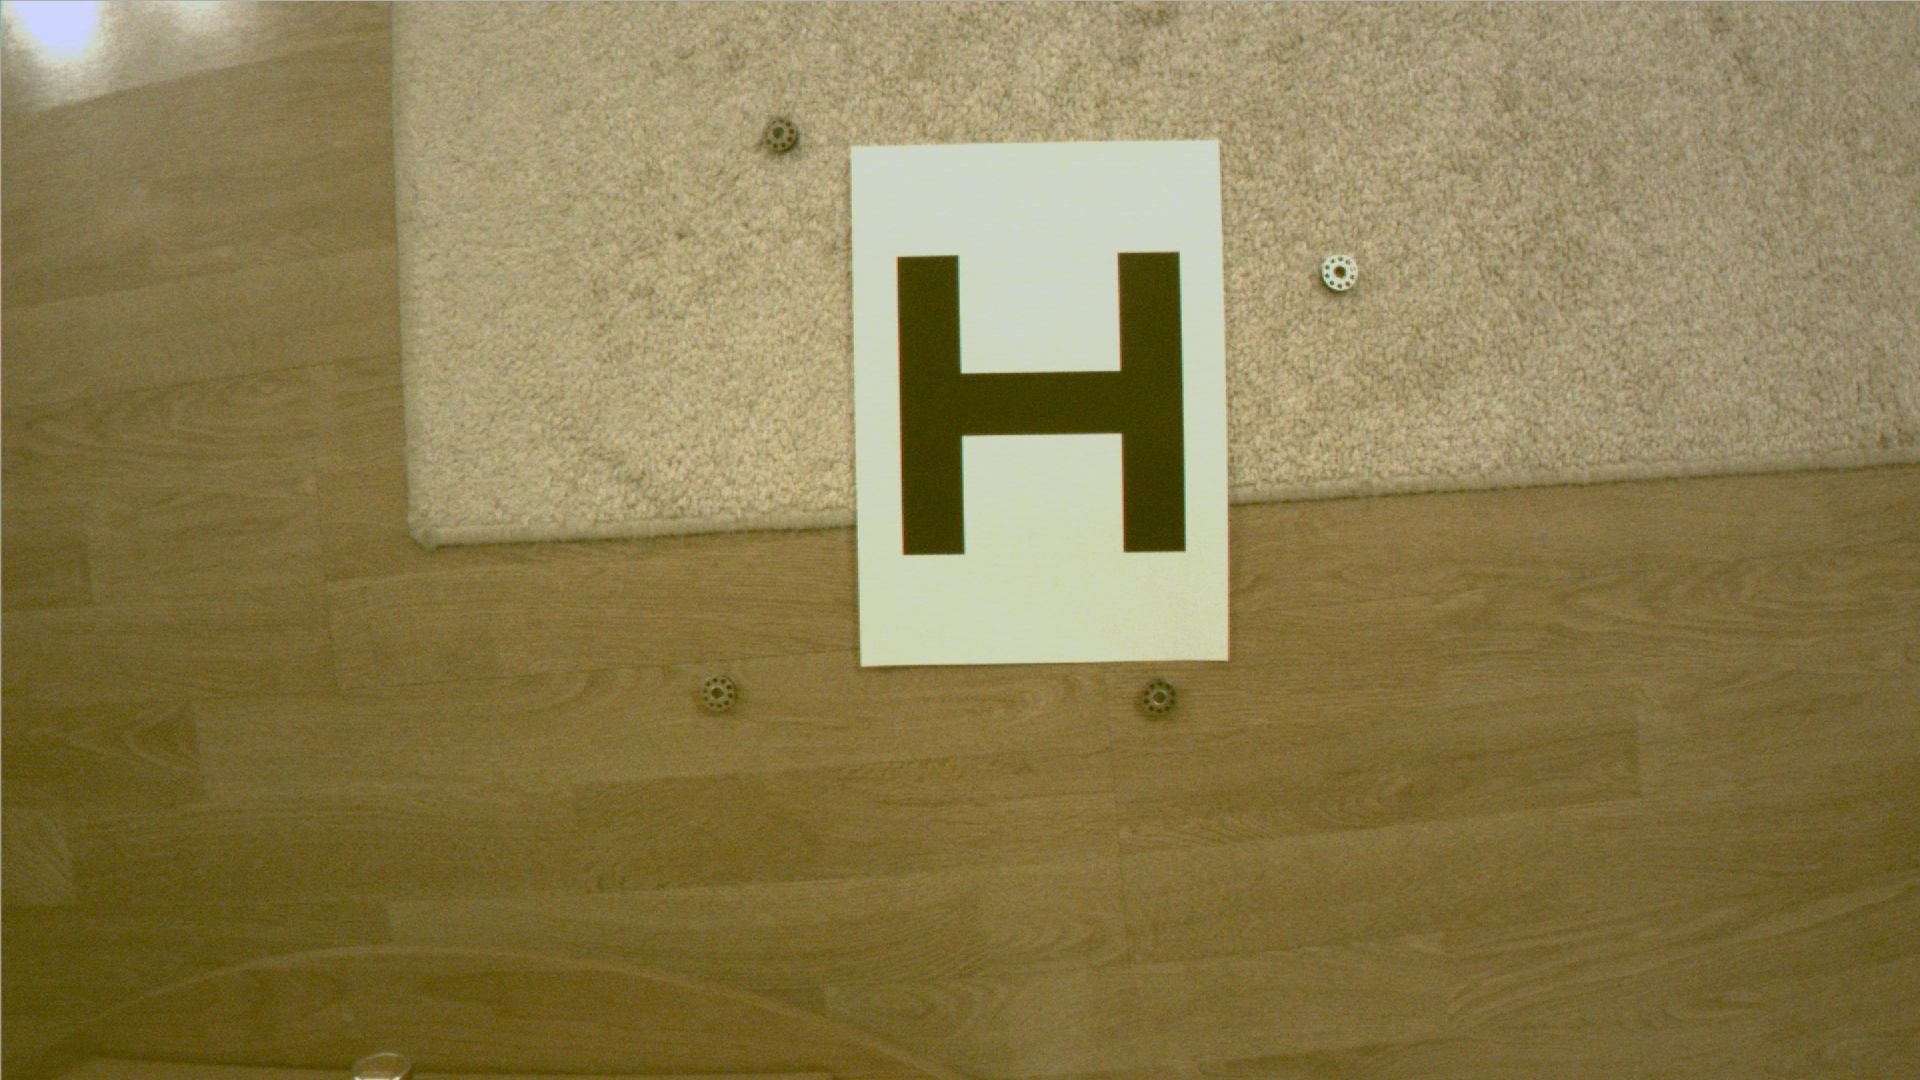
\includegraphics[width=\textwidth]{h.jpg}
	\caption{Obraz oryginalny}
	\label{fig:h}
\end{figure}
\begin{figure}[h]
	\centering
	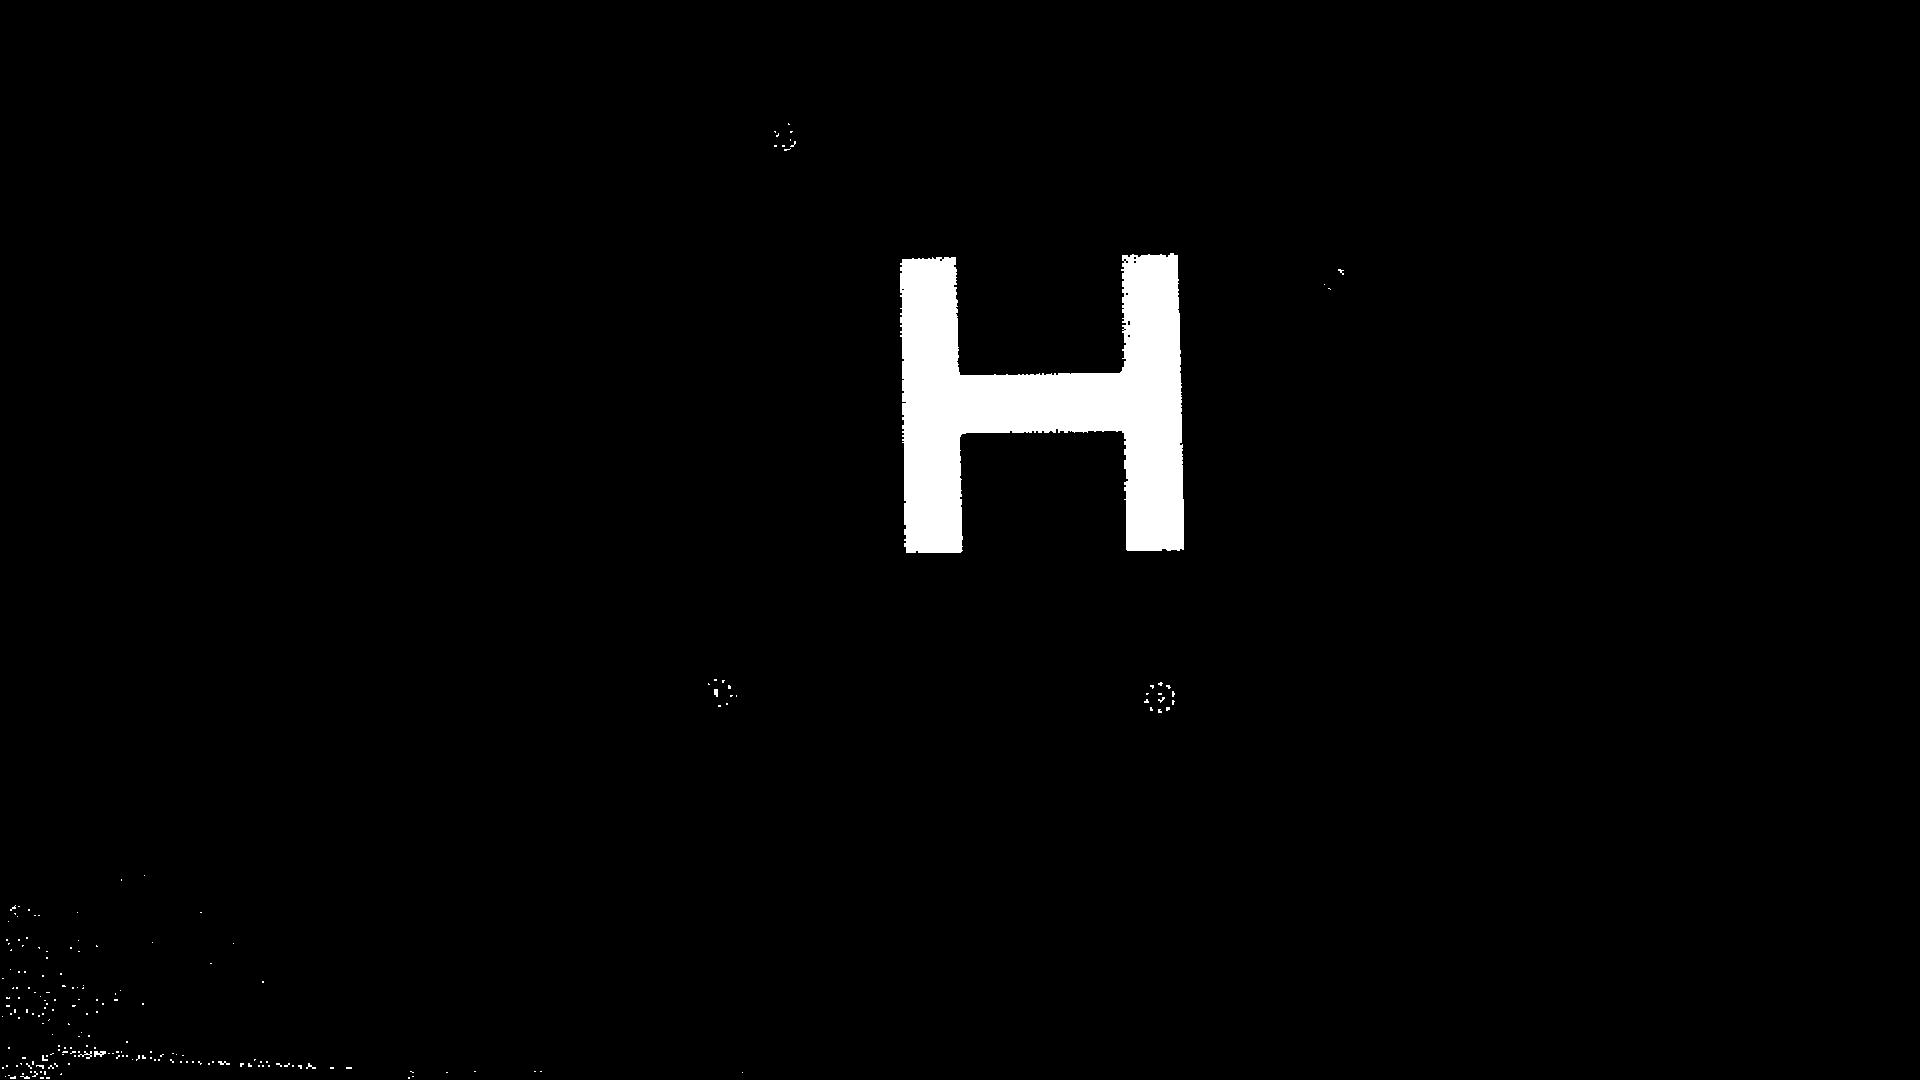
\includegraphics[width=\textwidth]{bin.jpg}
	\caption{Obraz po binaryzacji}
	\label{fig:bin}
\end{figure}
\begin{figure}[h]
	\centering
	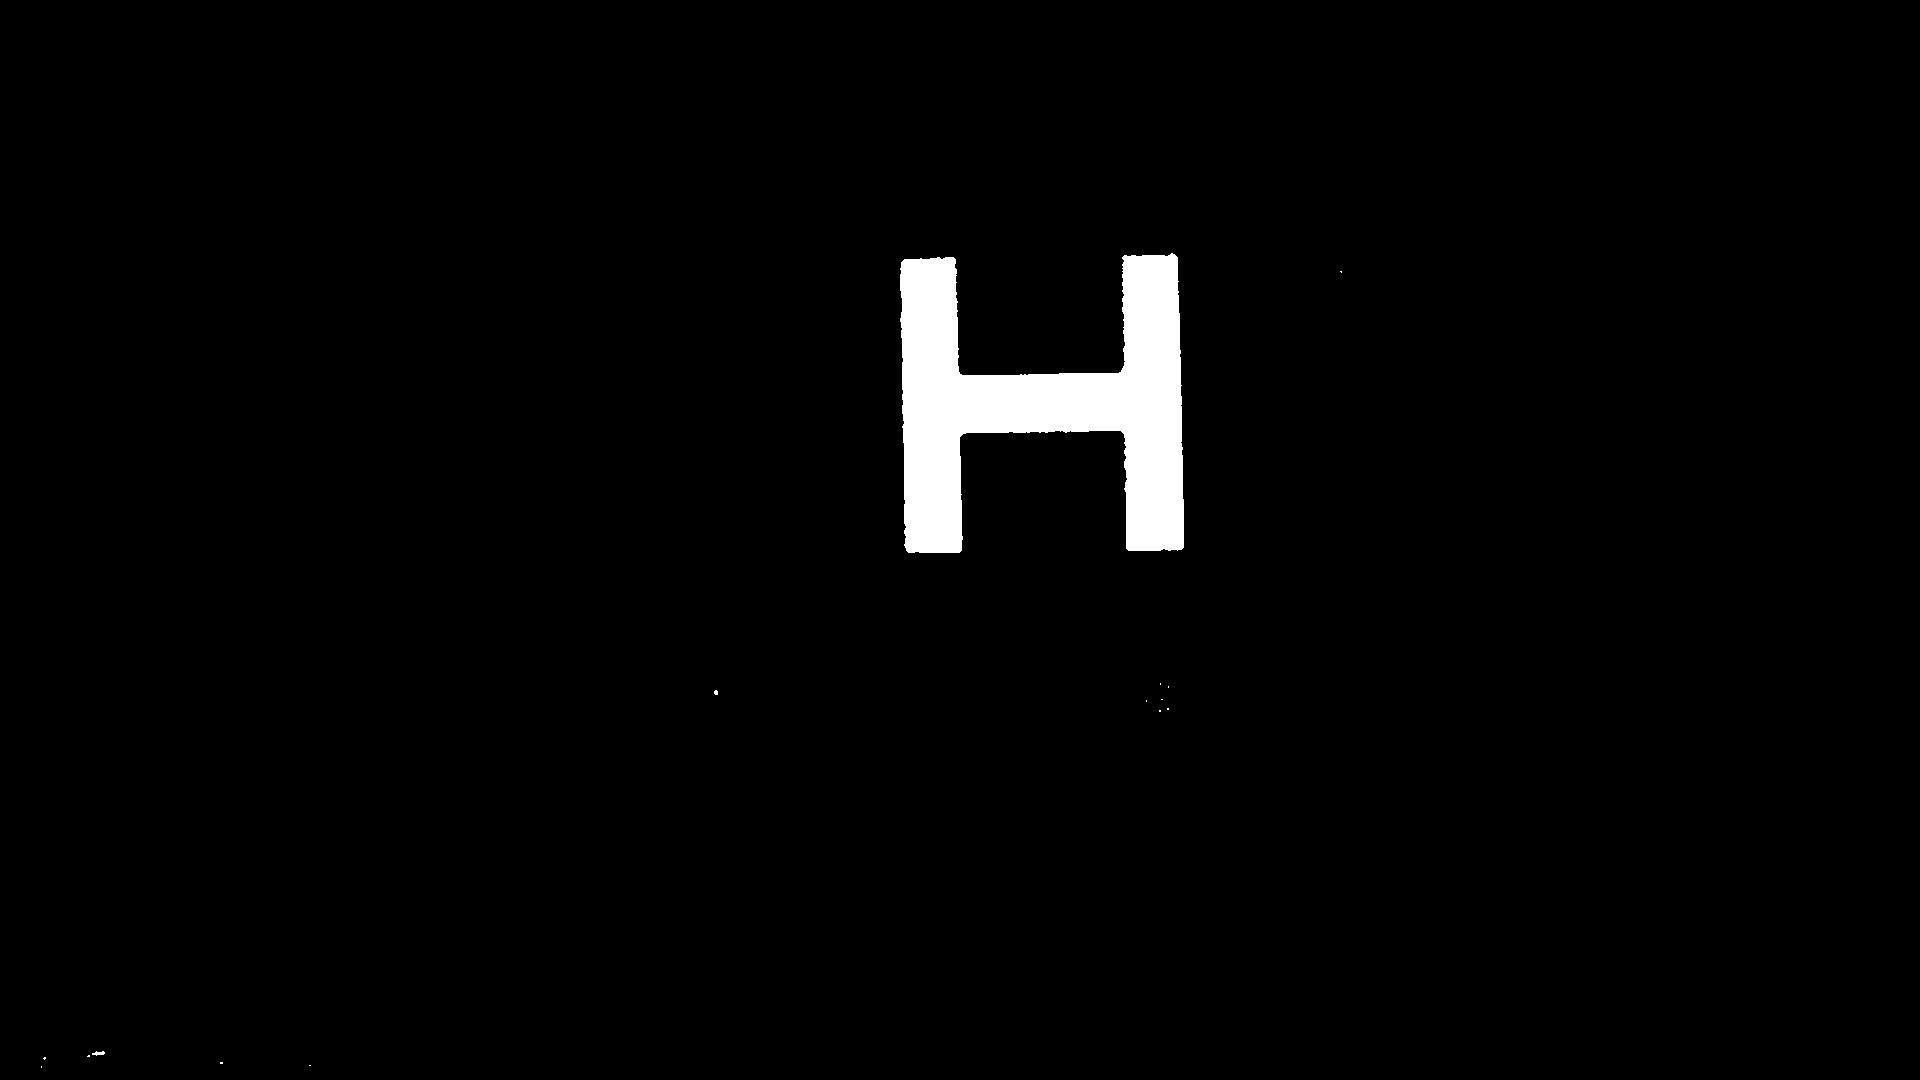
\includegraphics[width=\textwidth]{median.jpg}
	\caption{Obraz po medianie}
	\label{fig:median}
\end{figure}
\begin{figure}[h]
	\centering
	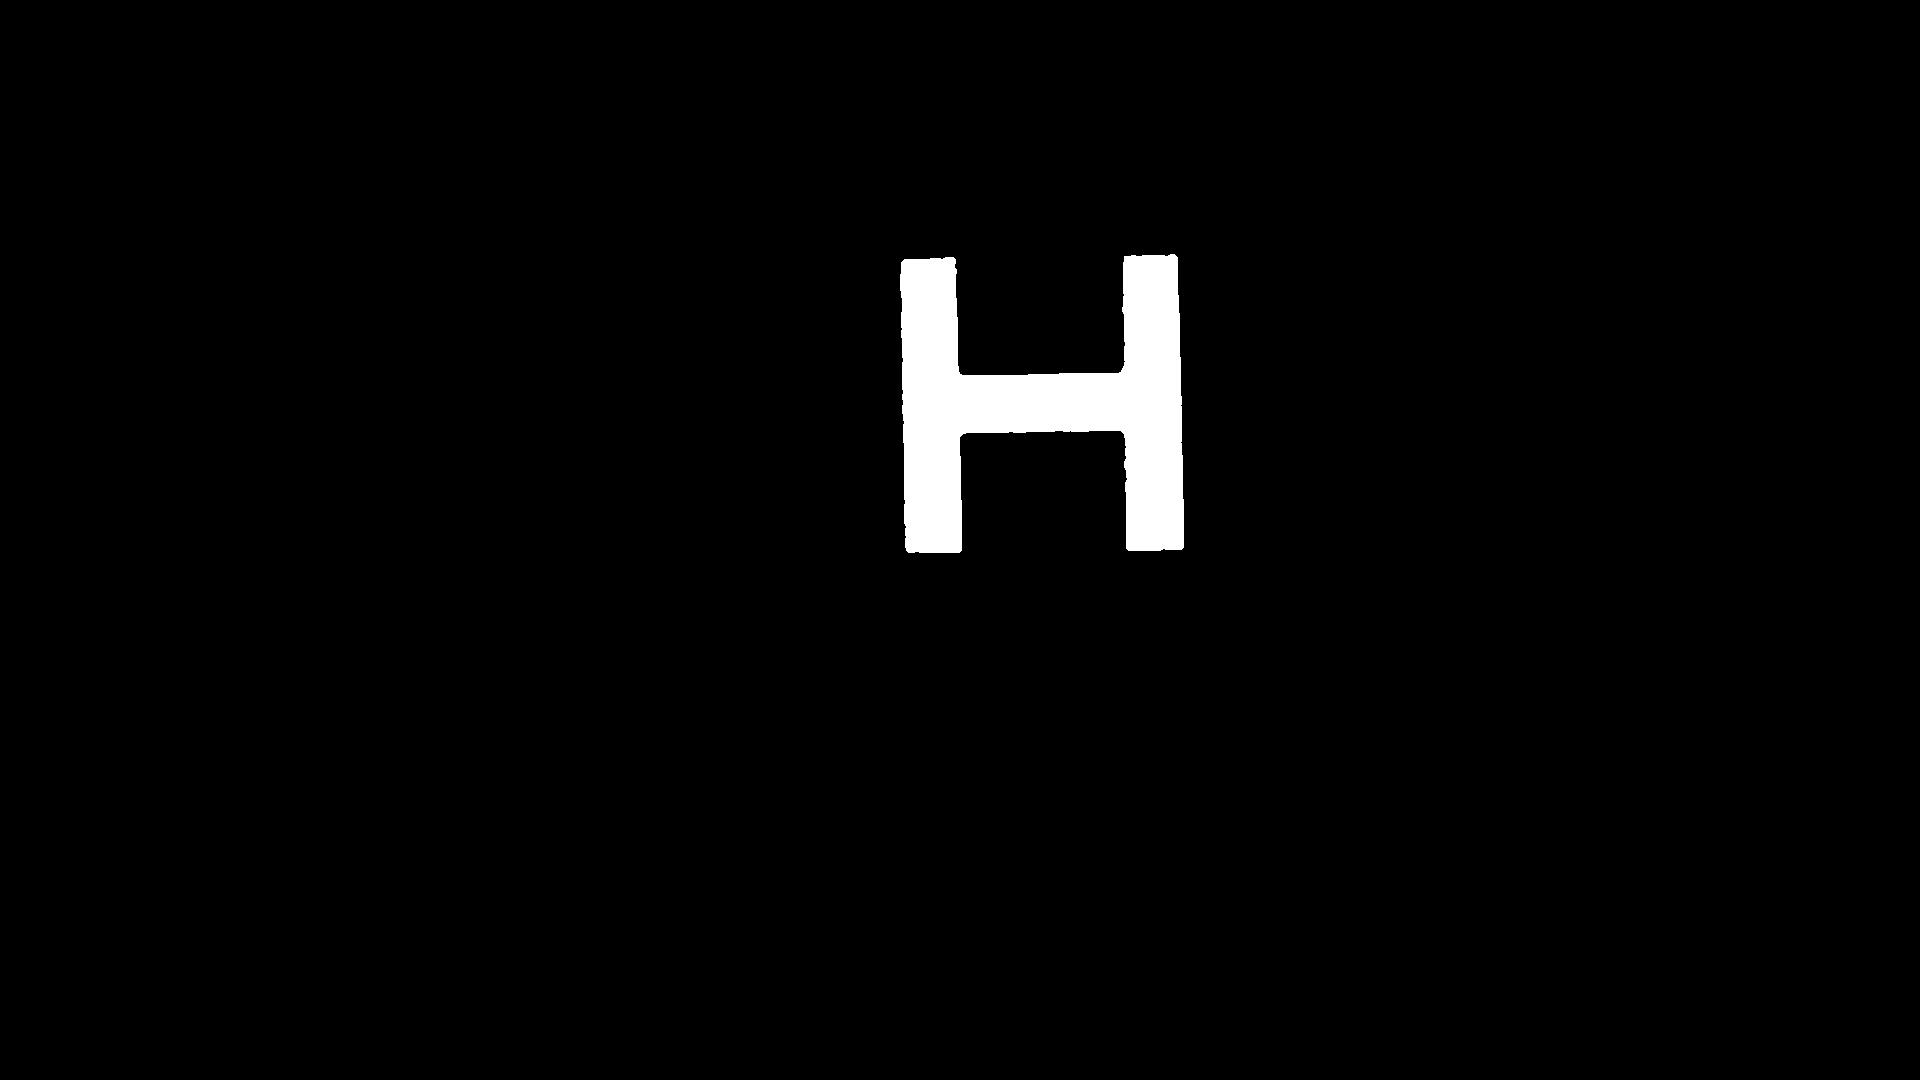
\includegraphics[width=\textwidth]{opened.jpg}
	\caption{Obraz po otwarciu}
	\label{fig:opened}
\end{figure}
\begin{figure}[h]
	\centering
	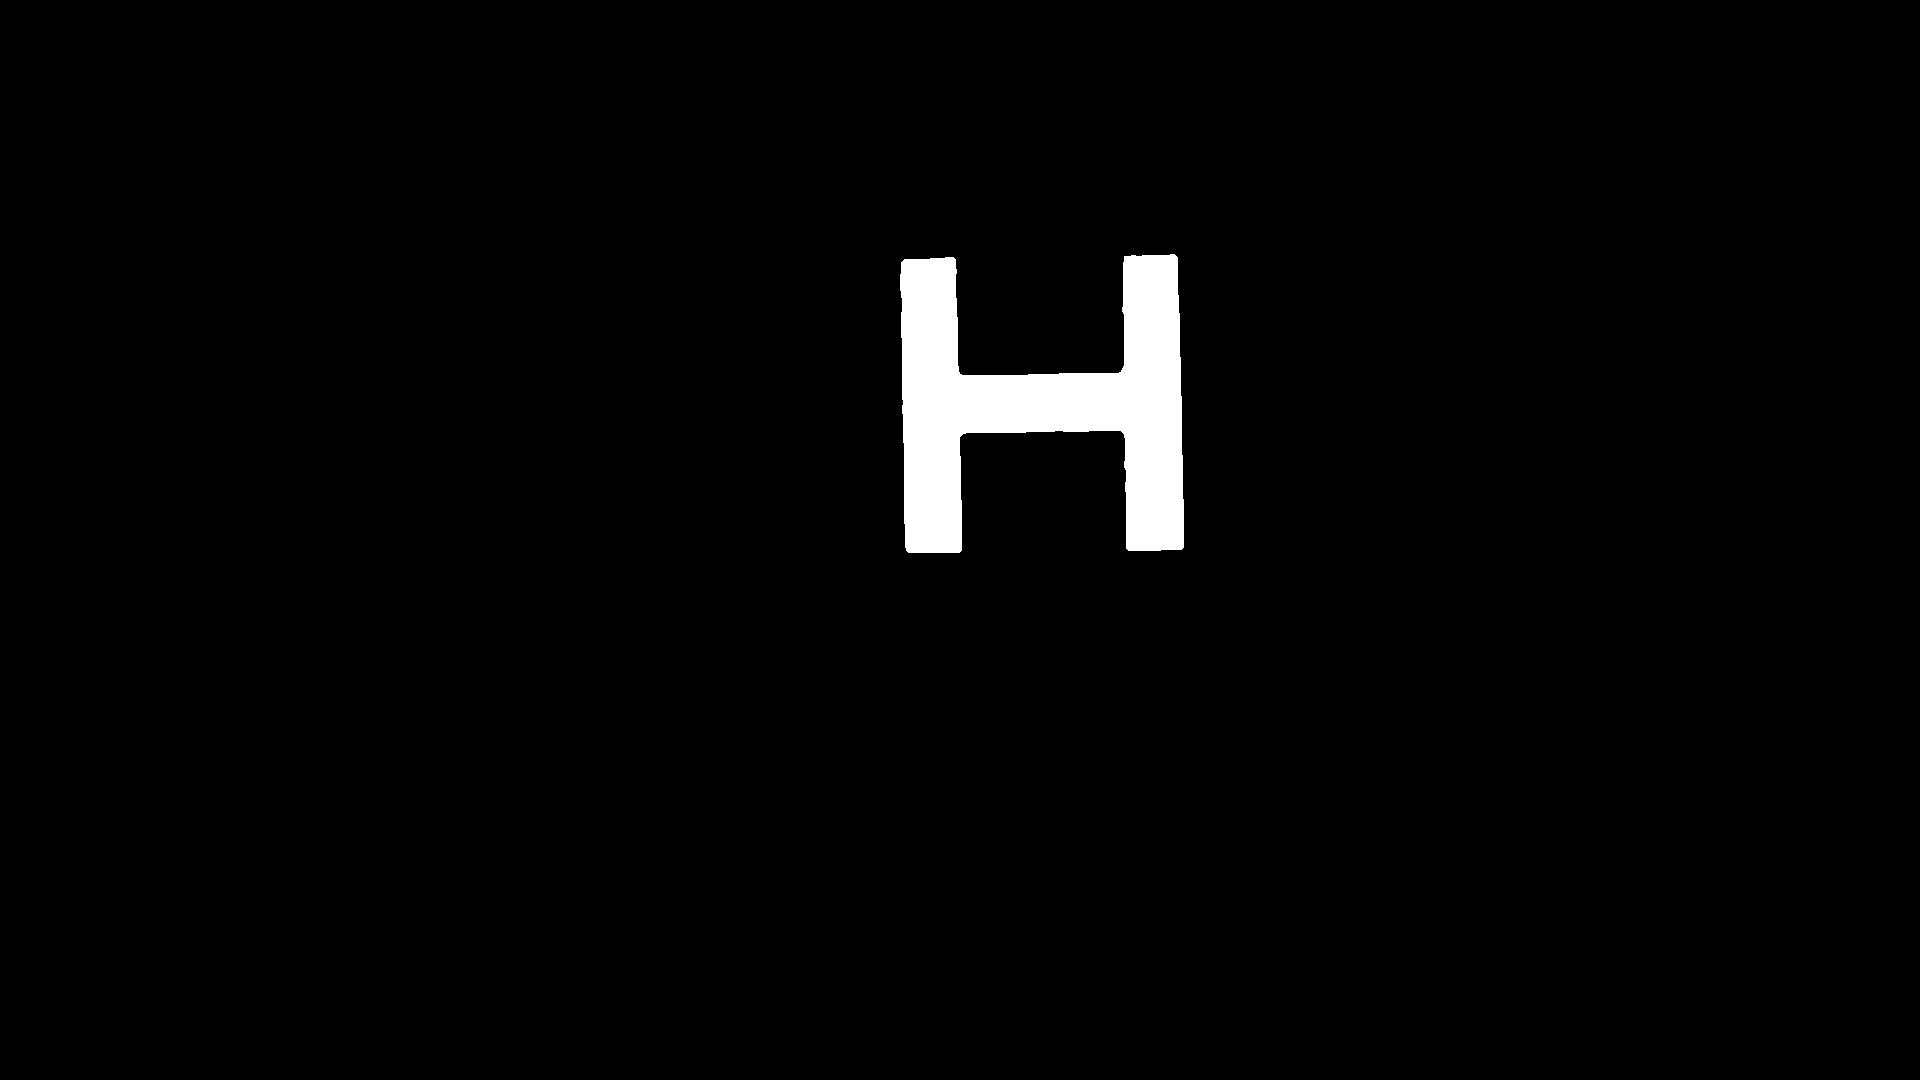
\includegraphics[width=\textwidth]{closed.jpg}
	\caption{Obraz po zamknięciu}
	\label{fig:closed}
\end{figure}
\section{Test regulacji położenia drona}
\label{sec:test_regulacji_polozenia_drona}
--- Test będzie polegał na zadawaniu prędkości w x i y proporcjonalnej do liczby pikseli dzielącej środek obrazu od aktualnego położenia znacznika. Celem będzie doprowadzenie do sytuacji stabilnego unoszenia drona nad znacznikiem. Rejestrowanie uchybu w x i y i ich zapis na kartę SD pozwoli na sporządzenie wykresów tych wartości w czasie.
\section{Lądowanie na nieruchomym lądowisku}
\label{sec:ladowanie_na_nieruchomym_ladowisku}
--- Do poprzedniego testu zostanie dodana funkcjonalność lądowania.
%---------------------------------------------------------------------------
=======

>>>>>>> 65f53b1db22d3a9ab1904ccaf9af33bb2165b4c7
%---------------------------------------------------------------------------
%---------------------------------------------------------------------------


%-------------------------------------------------------------------------
>>>>>>> 1f128f6bdf2d2b222fe828b89fbd544de01b028f
